\documentclass[threecolumns]{cheatsheet}
\usepackage{graphicx} % Required for inserting images
\usepackage{mathrsfs}
\usepackage{tikz}
\usepackage{array}
\usepackage{amsfonts}
\usepackage{booktabs}
\usepackage{supertabular}
\usepackage{pdfpages}
\usepackage{pdflscape}

\title{Physik ZF MAVT 2026}
\author{Wyss Stephan Physik ZF MAVT 2026}
\date{March 2026}

\raggedcolumns

\begin{document}
	
	% Manually start the layout structure here!
	\begin{multicols*}{3}
		\begin{adjustwidth}{1mm}{1mm}
			
			\section{Das elektrische Feld I}
\begin{flushleft}
\subsection{Definition: Elektrische Ladung}
Diskrete \textbf{Ladungsverteilung} (nicht kontinuierliche)\\
Die \textbf{elektrische Ladung} ist quantifiziert, d.h sie tritt als ganzzahliges vielfaches von $\textbf{e}$ auf
\[
    e \approx 1.602 \cdot 10^{-19} \ \text{C} \: [Coulomb]
\]\[
	-e \: \hat{=} \ \text{Ladung eines Elektrons}
\]\[
	e \: \hat{=} \ \text{Ladung eines Protons}
\]
Bei allen Prozessen ist die Gesamtladung vor \& nach der Wechselwirkung identisch

\subsection{Definition Elektrische Leiter \& nicht Leiter}
\textbf{Elektrische Leiter:} Stoffe, in denen sich ein Teil der Elektronen frei bewegen kann. \\
\textbf{Nichtleiter/Isolatoren:} Stoffe, in denen sich Elektronen nicht frei bewegen können. \\
Als \textbf{"Erde"} bezeichnet man einen Leiter der eine unbegrenzte Menge an Ladung auf- oder abgeben kann.

\subsection{Das Coulomb'sche Gesetz}
\begin{formulabox}
    \[\Vec{F} = \frac{1}{4\pi\epsilon_0}\frac{q_1 q_2}{r^2}\hat{e}_r\]
\end{formulabox}
\[
	|\Vec{F}_C|=  F_C = \frac{1}{4\pi\epsilon_0}\frac{e^2}{r^2} ,\  
	|\Vec{F}_G|=  F_G = \Gamma\frac{m_p m_e}{r^2}
\]
$F_G = $ Gravitationskraft mit $m_p = 1.67*10^{-27} ; m_e = 9.11*10^{-31}$ \\
\[
	\frac{F_C}{F_G} = \frac{1}{4\pi\epsilon_0}\frac{e^2}{\Gamma m_p m_e}
\]

\hspace{5mm} falls: $\frac{F_C}{F_G} \gg 1$, Gravitationseffekte sind vernachlässigbar.

\hspace{5mm} falls: $\frac{F_C}{F_G} \ll 1$, Gravitationseffekte überwiegen.

\subsection{Das Elektrische Feld}
Eine \textbf{Ladung} oder \textbf{Ladungsverteilung} erzeugt überall im Raum ein \textbf{$\Vec{E}-Feld$}, und durch dieses Feld, erfährt eine zweite Ladung eine Kraft

\textbf{Punktladung}: idealisierte Ladung ohne räumliche Ausdehnung

\textbf{Probeladung ($q_0$)}: Ladung, auf die durch andere Ladungen erzeugte Kräfte wirken


Feld am Ort der Probeladung $q_0$ ist definiert als $\Vec{E} = \frac{\Vec{F}}{q_0}$ ,\ [$\frac{Newton}{Coulomb}$]
\begin{formulabox}
    \[
    \Vec{E}_i = \frac{1}{4\pi\epsilon_0}\frac{q_i}{r_i^2}\hat{e}_{r,i}
    \]
\end{formulabox}
\begin{formulabox}
\[
    \Vec{E} = \sum_i\Vec{E}_i = \sum_i\frac{1}{4\pi\epsilon_0}\frac{q_i}{r_i^2}\hat{e}_{r,i}
\]    
\end{formulabox}

$\Rightarrow$ \text{wie für Kraft gilt für Felder das Superpositionsprinzip}

\subsection{Definition Elektrische Feldlinien}
\textbf{Elektrische Feldlinien} verlaufen in jedem Punkt tangential zum Feldvektor $\Vec{E}$

\textbf{Feldlinien} zeigen in Richtung der Kraft d.h. positiv $\rightarrow$ negativ

\textbf{Feldstärke} wird durch die \textbf{Dichte} der Feldlinien beschrieben

\subsection{Wirkung von elektrischen Felder auf Ladung}
Ein $\Vec{E}-Feld$, kann auf eine Punktladung eine Kraft und auf einen elektrischen Dipol eine Kraft und eine Drehmoment ausüben

Für die Beschleunigung eine geladenen Teilchen mit Masse $m$ in einem $\Vec{E}-Feld$ gilt:
\begin{formulabox}
\[
    \Vec{a} = \frac{\Vec{F}}{m} = \frac{q}{m}\Vec{E}
\]  
\end{formulabox}

Auf einen Dipol übt ein \textbf{homogene} äusseres $\Vec{E}-Feld$ keine resultierende Kraft aus. Das existierende Kräftepaar erzeugt aber ein \textbf{Drehmoment}.
\[
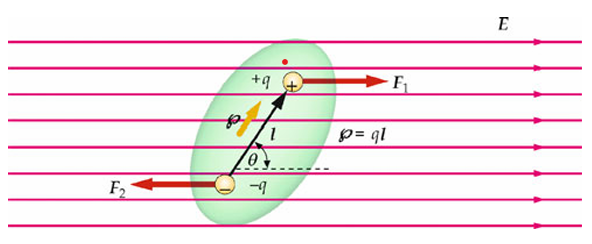
\includegraphics[width=0.5\linewidth]{Abbildungen Physik ZF/Dipol_Drehmoment.png}
\]
Das Drehmoment hat für jede der beiden Punktladungen des Dipols den Betrag:
\[
    |\Vec{F}||\Vec{l}|\sin{\theta} = |q \cdot \Vec{E}||\Vec{l}|\sin{\theta} = |\Vec{p}||\Vec{E}|\sin{\theta}
\]
In \textbf{Vektorform} gilt das \textbf{Kreuzprodukt}:
\begin{formulabox}
\[
    \Vec{M} = \Vec{p} \times \Vec{E}
\]
\end{formulabox}
Bei einer Drehung wird \textbf{Arbeit} verrichtet:
\[
    dW = - |\Vec{M}|d\theta = -|\Vec{p}||\Vec{E}|\sin{\theta}d\theta
\]\[
    dE_{pot} = -dW = |\Vec{p}||\Vec{E}|\sin{\theta}d\theta
\]
\textbf{Potentielle Energie} eins Dipols im $\Vec{E}-Feld$
\begin{formulabox}
\[
    E_{pot} = -|\Vec{p}||\Vec{E}|\cos{\theta} = -\Vec{p}\Vec{E}
\]
\end{formulabox}

\end{flushleft}
			\section{Das elektrische Feld II}
\begin{flushleft}
\subsection{Das Konzept der Ladungsdichte}
\[
    \text{Raumladungsdichte: } \rho = \frac{dq}{dV}
\]\[
    \text{(Ober-)Flächenladungsdichte: } \sigma = \frac{dq}{dA}
\]\[
    \text{Linienladingsdichte: } \lambda = \frac{dq}{dl}
\]

Zur Berechnung der \textbf{Gesamtladung}: Integration über Volumen, Flächen resp. Kurven

\subsection{Berechnung von \texorpdfstring{$\Vec{E}$}{E}  mit dem Coulomb'schen Gesetz}

Ansatz: $dp = \rho dV$ wird als Punktladung betrachtet.
\[
\Rightarrow \text{$d\Vec{E} = \frac{1}{4\pi\epsilon_0}\frac{dq}{r^2}\hat{e}_r$}
\]
\begin{formulabox}
\[
    \Vec{E} = \int d\Vec{E} = \int_V \frac{1}{4\pi\epsilon_0}\frac{dq}{r^2}\hat{e}_r
\]
\end{formulabox}
\subsection{Das Gauss'sche Gesetz}

\textbf{Aussage:} Die Differenz aus der Anzahl der eine Oberfläche verlassenden und der in die Oberfläche eintrettenden Feldlinien ist proportional zu der von der Oberfläche eingeschlossenen \textbf{Gesamtladung}


\textbf{elektricher Fluss} für eine Ebenefäche mit beliebiger Orientierung:
\[
    \Phi_E = \Vec{E}\cdot\Vec{A} = \Vec{E}\cdot A\hat{n}
\]
Allgemein für den Gesamtfluss $\Phi_E$ gilt:
\begin{formulabox}
\[
    \Phi_E: \lim_{ \Delta A_i \to O} \sum_i \Vec{E}_i \Delta \Vec{A_i}  = \int_A \Vec{E}d\Vec{A} 
\]
\end{formulabox}
Mathematische Formulierung durch das Kreisintegral (geschlossene Oberfläche)
\begin{formulabox}
\[
    \Phi_E = \oint_A \Vec{E}d\Vec{A}
\]
\end{formulabox}
\textbf{Gauss'sches Gesetz}
\begin{formulabox}
\[
    \Phi_E = \oint_A \Vec{E}d\Vec{A} = \oint_A E_n dA = \frac{q_{innen}}{\epsilon_0} \hspace{1cm}  EA = \frac{Q}{\epsilon_0}
\]
\end{formulabox}


\subsection{Berechnung von \texorpdfstring{$\Vec{E}$}{E} mit dem Gauss'schen Gesetz}
\vspace{-1em}
\begin{multicols}{2}
\centering
   \textbf{$\Vec{E}$ für dünne Kugelschale:}
\begin{formulabox}
    \[
    \Vec{E}_r = \frac{1}{4\pi\epsilon_0}\frac{q}{r^2} \hspace{3mm}, (r > r_k)
    \]\[
    \Vec{E}_r = 0 \hspace{3mm}, (r < r_k)
    \]
\end{formulabox}

    \textbf{$\Vec{E}$ für homogen geladene Vollkugel:}
\begin{formulabox}
    \[
        \Vec{E}_r = \frac{1}{4\pi\epsilon_0}\frac{q}{r^2} \hspace{3mm}, (r > r_k)
    \]
    \[
        \Vec{E}_r = \frac{1}{4\pi\epsilon_0}\frac{q}{r_k^2}r \hspace{3mm}, (r < r_k)
    \]
\end{formulabox}
 
\end{multicols}

    \begin{center}
    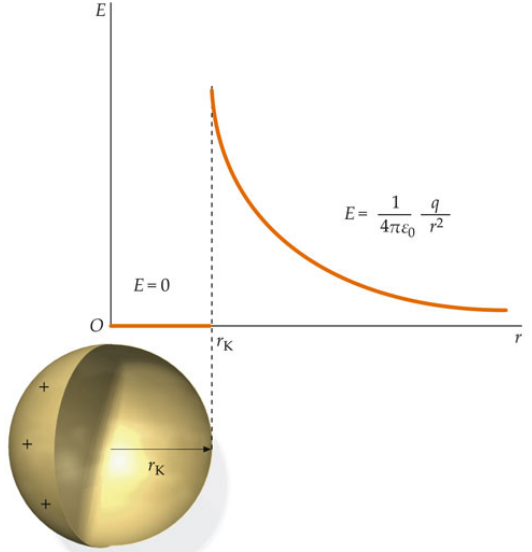
\includegraphics[width=0.34\linewidth]{Abbildungen Physik ZF/Gaussschens_Gesetz_dünne_Kugelschale.png}
    \hspace{5mm}
    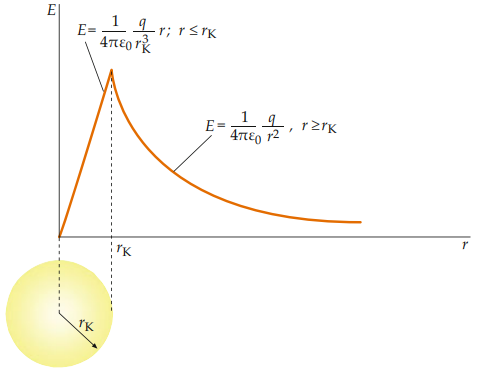
\includegraphics[width=0.45\linewidth]{Abbildungen Physik ZF/Gaussschens_Gesetz_Vollkugel.png}

    $\Vec{E}-Feld$ bei dünner Kugelschalen ist innerhalb immer = 0
    \end{center}

\subsection{Diskontinuität von \texorpdfstring{$E_n$}{En}}

\begin{center}
Unabhängig von der Form der Obergläche gilt:
\end{center}
\begin{formulabox}
    \[
    \Delta E_n = \frac{\sigma}{\epsilon_0}
    \]
\end{formulabox}
\begin{formulabox}
    \[
    \Delta E_n = E_{n,+} - E_{n,-} = \frac{\sigma}{2\epsilon_0} - \left(-\frac{\sigma}{2\epsilon_0}\right) = \frac{\sigma}{\epsilon_0}
    \]
\end{formulabox}
\subsection{Ladung \& Feld auf Leiteroberfläche}
Im elektrostatischen Gleichgewicht ist die Ladungsdichte und das $\Vec{E}-Feld$ im inneren eines Leiters überall = 0. \\
Das $\Vec{E}-Feld$ unmittelbar ausserhalb der Oberfläche hat keine tangentiale Komponente, nur Normalkomponente senkrecht zur Oberfläche mit: $E_n = \frac{\sigma}{\epsilon_0}$

\subsection{Das elektrische Potenzial}

\begin{formulabox}
    \[
    dE_{pot} = -\Vec{F} \cdot d\Vec{s}
    \]
\end{formulabox}
Für eine Punktladung $q_0$ gilt:
\begin{formulabox}
    \[
    dE_{pot} = dE_{el} = -q_0\Vec{E}\cdot d\Vec{s}
    \]
\end{formulabox}
Die Änderung der pot. Energie pro Ladungseinheit ist als Potenzialdifferenz definiert:
\begin{formulabox}
    \[
    d\phi = \frac{dE_{pot}}{q_0} = \frac{dE_{pot}}{q_0} = -\Vec{E} \cdot \Vec{s}
    \]
\end{formulabox}
Die Potenzialänderung bei Verschiebung von a nach b ist:
\begin{formulabox}
    \[
    \Delta\phi = \phi_b - \phi_a = \frac{\Delta E_{el}}{q_0} = - \int_b^a \Vec{E} \cdot d\Vec{s}
    \]
\end{formulabox}
Man wählt das elektr. Potenzial und die elektr. Energie so, dass sie im gleichen Bezugspunkt = 0 sind.
\begin{formulabox}
    \[
    E_{el} = q_0 \phi \hspace{7mm} [\phi] = \frac{J}{C} = V
    \]
\end{formulabox}
Die Potenzialdifferenz zwischen zwei Punkten wird auch (elektr.) Spannung genannt. \\
Es gilt: Das $\Vec{E}-Feld$ zeigt in die Richtung, in die das Potenzial $\phi$ am schnellsten abnimmt.

\subsection{Das Potenzial eines Punktladungsystems}
Für Punktladungen gilt: $\Vec{E} = \frac{1}{4\pi\epsilon_0} \frac{q}{r^2}\hat{e}_r$ \hspace{6mm} (B: Bezugspunkt ; P: beliebiger Punkt)
\[
    \phi_P - \phi_B = - \int_B^P \Vec{E}\cdot d\Vec{s} = -\int_B^P\frac{1}{4\pi\epsilon_0}\frac{q}{r^2}\hat{e}_r \cdot d\Vec{s} = -\int_B^P\frac{1}{4\pi\epsilon_0}\frac{q}{r^2}dr 
\]
\[
    \phi_P - \phi_B = \frac{1}{4\pi\epsilon_0}\frac{q}{r_P} - \frac{1}{4\pi\epsilon_0}\frac{q}{r_B}
\]
\\

Konvention: Bezugspunkt B im Unendlichen $\Rightarrow r_B \rightarrow \infty$
\begin{formulabox}
    \[
    \phi = \frac{1}{4\pi\epsilon_0}\frac{q}{r} \hspace{5mm} \text{Das Coulomb-Potenzial}
    \]
\end{formulabox}
\begin{formulabox}
    \[
    E_{el} = q_0\phi = \frac{1}{4\pi\epsilon_0}\frac{q_0 q}{r} \hspace{4mm} \text{elektr. Energie einer Punktladung}
    \]
\end{formulabox}
\begin{formulabox}
    \[
    \phi = \sum_i \frac{1}{4\pi\epsilon_0}\frac{q_i}{r_i} \hspace{3mm} \text{Potenzial eines Systems mit Superposition}
    \]
\end{formulabox}
\subsection{Berechnung des elektrischen Felds aus dem Potenzial}
Es gilt: $d\phi = -\Vec{E}\cdot\ d\Vec{s}$\\
\hspace{5mm} falls: $d\Vec{s} \perp \Vec{E}$ ist $d\phi$ = 0\\
\hspace{5mm} falls: $d\Vec{s} \parallel \Vec{E}$ ist $d\phi$ = maximal
\\[1ex]
Das $\Vec{E}-Feld$ ist gleich dem Negativen des Gradientes des Potenzials $\phi$
\begin{formulabox}
    \[
    \Vec{E} = -\nabla\phi = -\left(\frac{\partial\phi}{\partial x}\hat{e}_x + \frac{\partial\phi}{\partial y}\hat{e}_y + \frac{\partial\phi}{\partial z}\hat{e}_z\right)
    \]
\end{formulabox}

\subsection{Berechnung von \texorpdfstring{$\phi$}{phi} kontinuierlicher Ladungsverteilung}
Aus dem Superpositionsprinzip folgt: $\phi = \int \frac{1}{4\pi\epsilon_0}\frac{dq}{r}$\\
Annahme: Im Unendlichen Abstand von den Ladungen ist $\phi$ = 0.
\\[2ex]
\textbf{$\phi$ innerhalb \& ausserhalb einer homogenen geladenen Kugelschale:}
\begin{formulabox}
    \[
    \phi = -\int_{\infty}^{r_P} \frac{1}{4\pi\epsilon_0}\frac{q}{r^2}dr = \frac{1}{4\pi\epsilon_0}\frac{q}{r_P} \hspace{5mm} (r_P \geq r_K)
    \]
\end{formulabox}
$\Vec{E}$ innerhalb = 0; $\phi$ im inneren $\neq$ 0 !
\begin{formulabox}
    \[  
    \phi = -\int_{\infty}^{r_K} \frac{1}{4\pi\epsilon_0}\frac{q}{r^2}dr -\int_{r_K}^{r_P} \text{0} \ dr = \frac{1}{4\pi\epsilon_0}\frac{q}{r_K} \hspace{5mm} (r_P < r_K) 
    \]
\end{formulabox}

\subsection{Äquipotenzialflächen}
In einer Äquipotenzialfläche ist $\phi$ konstant. Feldlinien stehen immer senkrecht zu den Äquipotentialflächen.\\[1ex]
Jede Oberfläche eines Leiters ist eine Äquipotenzialfläche:
\[
    \phi = \frac{1}{4 \pi \epsilon_0}\frac{q}{r} \rightarrow q = 4 \pi r^2 \sigma \rightarrow \phi = \frac{1}{4 \pi \epsilon_0}\frac{4 \pi r^2 \sigma}{r} = \frac{r \sigma}{\epsilon_0} \rightarrow \sigma = \frac{\phi \epsilon_0}{r}
\]

\subsection{Die elektrische Energie}
Körper, die sich abstossen, besitzen eine höhere potenzielle Energie, wenn die näher beieinander sind. \\[1ex]
$\Rightarrow$ Arbeit wird verrichtet, um sie näher zu bringen \\[1ex]
Sich anziehende Körper haben die höchste potenzielle Energie, wenn sie weit voneinander entfernt sind.
\[
    \Rightarrow Arbeit: W = q \phi = q \frac{1}{4 \pi \epsilon_0}\frac{q}{r} = \frac{1}{4 \pi \epsilon_0}\frac{q_1 \cdot q_2}{r}
\]
\begin{formulabox}
    \[
     E_{el} = \frac{1}{2} \sum q_i \phi_i \hspace{3mm} \text{elektrische Energie eines Punktladungsystems}
    \]
\end{formulabox}

\end{flushleft}
			\section{Die Kapazität}

Als Kapazität wird das Verhältnis der Ladung $q$, die sich auf einem Leiter befindet, zu seiner elektrischen Spannung $U$ gegenüber einem Bezugspunkt definiert:
\[
    \text{Spannung:} \ U = \phi_B - \phi_A
\]\[
    \text{Kapazität:} \ C = \frac{q}{U}
\]
Einheit [C]: = Farad = F = $\frac{C}{V}$ = $\frac{Coulomb}{Volt}$

\subsection{Kondensatoren}
Ist eine Anordung von zwei Leiter, die beide eine gleich grosse, aber entgegengesetzte Ladung tragen können.\\[1ex]
Ladungen sind: $+q$ und $-q$ \\[2ex]
\textbf{Kapazität eines Kondensators:} 
\[
    C = \frac{q}{U} \ ; \ q \ \text{als Ladung auf einem Leiter und} \ U \ \text{als Spannung zwischen den Leiter}
\]

\textbf{Der Plattenkondensator}
Es gilt:
\[
    U = E \cdot d = \frac{\sigma}{\epsilon_0} \cdot d = \frac{q \cdot d}{\epsilon_0 \cdot A}
\]
$E = \frac{\sigma}{\epsilon_0}$: als $\Vec{E}-Feld$ zwischen den Oberflächen \\[1ex]
$d$: als Abstand zwischen den Platten \\[1ex]
$\sigma = \frac{q}{A}$: als Flächenladungdichte, $A$: Fläche der Platte \\[2ex]
\textbf{Kapazität eines Plattenkondensators:}
\begin{formulabox}
\[
     C = \frac{q}{U} = \frac{q}{(\frac{q \cdot d}{\epsilon_0 A})} = \frac{\epsilon_0 A}{d}
\]
\end{formulabox}
\textbf{Kapazität eines Zylinderkondensators:}
\begin{formulabox}
    \[
    C = \frac{q}{U} = \frac{2 \pi \epsilon_0 l}{\ln(\frac{r_2}{r_1})}
    \]
\end{formulabox}

\subsection{Speichern von elektrischer Energie}
Arbeit wird während dem Ladevorgang eines Kondensators verrichtet und kann als elektrische Energie gespeichert werden. \\[1ex]
Der Gesamtzuwachs an Energie wird wiefolgt beschrieben: 
\[
    E_{el} = \int_0^q dE_{el} = \int_0^q \frac{q'}{C}dq' = \frac{1}{C}\int_0^q q' dq' = \frac{1}{2}\frac{q^2}{C}
\]
\textbf{Die im Kondensator gespeicherte Energie:}
\begin{formulabox}
    \[
    \Rightarrow E_{el} = \frac{1}{2}\frac{q^2}{C} = \frac{1}{2}qU = \frac{1}{2}CU^2
    \]
\end{formulabox}

Definiert man $w_{el}$ als Energiedichte (Energie pro Volumen) so folgt: \\[1ex]
\textbf{Energiedichte des elektrischen Felds:}
\begin{formulabox}
    \[
        w_{el} = \frac{\text{Energie}}{\text{Volumen}} = \frac{1}{2}\epsilon_0 E^2
    \]
\end{formulabox}

\subsection{Kondensatoren, Batterien \& elektrische Stromkreise}
Über alle Parallelgeschaltenen Bauelementen in elektr. Stromkreisen, herrt die gleiche Spannung. \\[1ex]
Für die gespeicherte Gesamtladung gilt:
\[
    q = q_1 + q_2 = C_1 U + C_2 U = U(C_1 + C_2)
\]
Ein einzelner Kondensator mit gleicher Wirkung wie die zusammen geschaltenen nennt man Ersatzkapazität:\\[3ex]
Für \textbf{Parallelschaltung} gilt:
\[
    C = \frac{q}{U} = \frac{q_1 + q_2}{U} = \frac{q_1}{U} + \frac{q_2}{U} = C_1 + C_2
\]
\textbf{Ersatzkapazität für parallel geschaltete Kondensatoren}
\begin{formulabox}
    \[
        \Rightarrow C_{eq} = C_1 + C_2 + ... + C_i
    \]
\end{formulabox}

Für \textbf{Reihen-/ Serienschaltung} gilt:
\[
    U = \phi_A - \phi_B = U_1 + U_2 = \frac{q}{C_1} + \frac{q}{C_2} = q\left( \frac{1}{C_1} + \frac{1}{C_2} \right)
\]
\textbf{Ersatzkapazität für in Reihe geschaltete Kondensatoren}
\begin{formulabox}
    \[
        \Rightarrow C_{eq} = \left( \frac{1}{C_1} + \frac{1}{C_2} + ... + \frac{1}{C_i} \right)^{-1}
    \]
\end{formulabox}

\subsection{Dielektrika}
Dielektrikas sind nichtleitende Matrielien (z.B Holz, Glas, Plexiglas, etc.) \\[2ex]

\textbf{Kapazitäterhöhung} durch ein Dielektrikum: \\[1ex]
$\Rightarrow \Vec{E} = \frac{\Vec{E}_0}{\varepsilon_{rel}}$ \\[1ex]
Dielektrikum schwächt $\Vec{E}-Feld \rightarrow$ gleiche Ladung, kleinere Spannung $\rightarrow$ höhere Kapazität. \\[1ex]
$\varepsilon_{rel}$: hängt vom Dielektrikum ab, ist eine Matrielkonstante \\[2ex]
\begin{formulabox}
    \[
        \Rightarrow U = E \cdot d = \frac{E_0 \cdot d}{\varepsilon_{rel}} = \frac{U_0}{\varepsilon_{rel}}
    \]  
\end{formulabox}
\begin{formulabox}
    \[
        \Rightarrow C = \frac{q}{U} = \varepsilon_{rel}\frac{q}{U_0} = \varepsilon_{rel} \cdot C_0
    \]
\end{formulabox}

\textbf{gespeicherte Energie und die Energiedichte:}
\begin{formulabox}
    \[
        E_{el} = \frac{1}{2}CU^2 = \frac{1}{2}\varepsilon_{rel}\epsilon_0 E^2 A d
    \]
    \[
    w_{el} = \frac{1}{2}\varepsilon_{rel}\epsilon_0 E^2
    \]
\end{formulabox}
			\section{Elektrischer Strom - Gleichstromkreise}

Der Fluss von elektrischen Ladungen wird als \textbf{elektrischer Strom} bezeichnet.

\subsection{elektrischer Strom und die Bewegung von Ladung}
\textbf{Definition Strom:}\\
Die Rate, mit der elektrische Ladung durch einen Leiterquerschnitt fliesst.
\[
    I = \frac{\Delta q}{\Delta t} \hspace{3mm} [I] = \text{Ampère} = A = \frac{C}{s}
\]
\textbf{Konvention:} Strom ist positiv, wenn er durch positive Ladungsträger in positiver Richtung erzeugt wird, resp. durch negative Ladungsträger in negative Richtung.
\[
    \Delta q = q\left( \frac{n}{v} \right) \cdot A \cdot v_d \cdot \Delta t \hspace{5mm} v_d: \text{Driftgeschwindigkeit}
\]
\begin{formulabox}
    \[
        \Rightarrow I = \frac{\Delta q}{\Delta t}  = q\left( \frac{n}{v} \right) \cdot A \cdot v_d
    \]
\end{formulabox}
\textbf{Stromdichte:}
\begin{formulabox}
    \[
        \Vec{j} = q \left( \frac{n}{v}\right) \cdot \Vec{v_d}
    \]
\end{formulabox}
\textbf{Strom durch eine Fläche $\Vec{A}$:}
\begin{formulabox}
    \[
        I = \int_A \Vec{j} \cdot d \Vec{A} = \int_A \Vec{j} \cdot \hat{e_n} \cdot dA
    \]
\end{formulabox}

\subsection{Widerstand und Ohm'sches Gesetz}
\textbf{Ohm'sches Gesetz}
\begin{formulabox}
    \[
    U = R \cdot I \hspace{1mm} ; \hspace{5mm} R = \text{konst.}
    \]
\end{formulabox}
\textbf{Definition des Widerstand $R$:}
\[
    R = \frac{U}{I} \hspace{3mm} [R] = \text{Ohm} = \Omega = \frac{V}{A}
\]
\textbf{Widerstand für leitfähigen Draht} mit $r$ als spezifischer Widerstand:
\[
    R = r \cdot \frac{l}{A} \hspace{3mm}
\]
\textbf{Vektorielle Form} des Ohm'schen Gesetzes:
\begin{formulabox}
    \[
        \Vec{j} = \sigma \Vec{E}
    \]
\end{formulabox}
$\sigma$ als elektr. Leitfähigkleit $\sigma = \frac{1}{r} = \frac{1}{\rho}$ \hspace{3mm} $\left[ \frac{S}{m}\right] = \left[ \frac{1}{\Omega m}\right]$
\[
    I = \sigma EA = \frac{1}{r} \frac{E \cdot l \cdot A}{l} = \frac{1}{r} U \frac{A}{l} = \frac{U}{R}
\] \\[1ex]
\textbf{Temperaturabhängiger Widerstand:} \\
$r_0$ sei der spezifische Widerstand bei Temperatur $T_0$ (i.d.R bei 20°)
\[
    \alpha = \frac{\left(r-r_0\right) / r_0}{T - T_0} \hspace{5mm} \alpha = \text{Temperaturkoeffizient}
\]
\subsection{Energetische Betrachtung elektrischer Stromkreise}
Verlust von \textbf{potenzieller Energie $\Delta E_{el}$:}
\[
    \Delta E_{el} = \Delta q \left( \phi_B - \phi_A \right) = \Delta q (-U)
\]
\begin{formulabox}
    \[
    \Rightarrow -\frac{\Delta E_{el}}{\Delta t} = \frac{\Delta q}{\Delta t} U
 = IU    \]
\end{formulabox}
Verlust von Energie $\Delta E_{el}$ wird in therm. Energie (Joul'sche Wärme) umgewandelt:
\\[1ex]
\[
    P = IU \hspace{5mm} \text{Im Leiterstück umgesetzte Leistung}
\] 
\\[1ex]
Für einen \textbf{Ohm'schen Widerstand} gilt:
\begin{formulabox}
    \[
        P = IU_R = RI^2 = \frac{U_R^2}{R}
    \]
\end{formulabox}

\subsection{Spannungsquellen und Quellenspannung}
Spannungsquellen führen einem Stromkreis elektrische Energie hinzu. \\
\textbf{Leistung einer Spannungsquelle:}
\[
    P = \frac{(\Delta q) U_Q}{\Delta t} = I U_Q
\] 
\\[1ex]

\textbf{Ideale Spannungsquellen} weisen an den Polen, unabhängig vom Stromfluss, immer dieselbe Quellspannung $U_Q$ auf:
\[
    I = \frac{U_Q}{R}
\]
\\[1ex]
\textbf{Reale Spannungsquellen} weisen eine Klemmspannung $U_K$ auf mit $U_K \neq U_Q$:
\[
    \phi_A = \phi_B + U_Q - R_{in} \cdot I \ ; \hspace{5mm} R_{in} = \text{Innenwiderstand}
\]
\\[1ex]
\textbf{Klemmspannung:}
\begin{formulabox}
    \[
        \phi_A - \phi_B = U_Q - R_{in} \cdot I
    \]
\end{formulabox}
\[
    RI = \phi_A - \phi_B = U_Q - R_{in} I \rightarrow I = \frac{U_Q}{R + R_{in}}
\]
\\[1ex]
\textbf{In der Batterie gespeicherte Energie:}
\begin{formulabox}
    \[
        \Rightarrow E_{el} = q\cdot U_Q
    \]
\end{formulabox}

\subsection{Zusammenschalten von Widerständen}
Für \textbf{Parallelschaltung} gilt:
\[
    I = \frac{U_R}{R} = \frac{U_R}{R_1} + \frac{U_R}{R_2} + ... + \frac{U_R}{R_i} = U_R \left( \frac{1}{R_1} + \frac{1}{R_2} + ... + \frac{1}{R_i} \right)
\]
\textbf{Ersatzwiderstand für parallel geschaltete Widerstände}
\begin{formulabox}
    \[
       \Rightarrow R_{eq} = \left( \frac{1}{R_1} + \frac{1}{R_2} + ... + \frac{1}{R_i} \right)^{-1}
    \]
\end{formulabox}

Für \textbf{Reihen-/ Serienschaltung} gilt:
\[
    U_R = U_1 + U_2 = R_1 I + R_2 I = I(R_1 + R_2)
\]
\textbf{Ersatzwiderstand für in Reihe geschaltete Widerstände}
\begin{formulabox}
    \[
       \Rightarrow R_{eq} = ( R_1 + R_2 + ... + R_i)
    \]
\end{formulabox}

\subsection{Die Kirchhoff'schen Regeln}
Anwendbar bei \textbf{stationärem (zeitunabhängigen)} Stromfluss. \\[1ex]
\hspace{5mm} \textbf{1. Knotenregel:} \\
\hspace{10mm} Summe aller hineinfliessenden Ströme ist \textbf{gleich} der Summe aller \\ \hspace{10mm} herausfliessenden
\\[2ex]
\hspace{5mm} \textbf{2. Maschenregel:} \\
\hspace{10mm} Summe aller Spannungen beim Durchlauf einer geschlossenen Schleife ist \\ \hspace{10mm} gleich \textbf{Null}
\\[2ex]

\subsection{RC-Schaltkreise}
Schaltungen mit Ohm'schem Widerstand R und Kondensator C. \\[2ex]

\textbf{Entladen eines Kondensators:} \\
Für $t = 0$ (Schalter geschlossen $\rightarrow$ entladen) gilt:
\[
    U_{C,0} = \frac{q_0}{C} 
\]
\hspace{5mm} \textbf{Strom durch $R$:}
\[
    I_0 = \frac{U_{C,0}}{R} =\frac{q_0}{RC} \rightarrow  I(t) = -\frac{dq(t)}{dt}
\]
\hspace{5mm} \textbf{Maschenregel:}
\[
    \frac{q(t)}{C} - RI(t) = 0 \rightarrow \frac{q(t)}{C} + R\frac{dq(t)}{dt} = 0 \rightarrow \frac{dq(t)}{dt} = - \frac{1}{RC}q(t)
\]
\\[1ex]
\begin{formulabox}
    \[
        q(t) = q_0 e^{-\frac{t}{RC}} \Rightarrow q_0 e^{-\frac{t}{\tau}} \hspace{5mm} \tau = RC
    \]
\end{formulabox}
\hspace{5mm} \textbf{Für dem Strom gilt:}
\begin{formulabox}
    \[
        I = -\frac{dq(t)}{dt} = \frac{q_0}{RC}e^{-\frac{t}{\tau}} = I_0 e^{-\frac{t}{\tau}}
    \]
\end{formulabox}

\textbf{Aufladen eines Kondensators:} \\
Für $t = 0$ (Schalter geschlossen $\rightarrow$ aufladen) gilt:
\\[1ex]
\hspace{5mm} \textbf{Maschenregel:}
\[
    U - I(t) R - \frac{q(t)}{C} = 0
\]
\hspace{5mm} Mit \textbf{Strom $I$:}
\[
    I(t) = \frac{dq(t)}{dt} \rightarrow U - R\frac{dq(t)}{dt} - \frac{q(t)}{C} = 0
\]
\begin{formulabox}
    \[
    q(t) = CU\left( 1 - e^{-\frac{t}{\tau}} \right) = q_E\left( 1 - e^{-\frac{t}{\tau}} \right) \hspace{5mm} q_E = \text{max. Ladung}
    \]
\end{formulabox}
\hspace{5mm} \textbf{Für den Strom gilt:}
\begin{formulabox}
    \[
        I(t) = \frac{dq(t)}{dt} = CU \left( \frac{1}{RC} \cdot e^{-\frac{t}{\tau}} \right) = \frac{U}{R}e^{-\frac{t}{\tau}} = I_Ae^{-\frac{t}{\tau}}
    \]
\end{formulabox}
\vspace{2ex}

\subsection{Energiebilanz beim Aufladen eines Kondensators}
Ladung $q_E = CU$ fliesst beim Aufladen durch die Batterie \\[1ex]
Dabei verrichtete Arbeit: $W = q_E \cdot U = CU^2$ \\[1ex]
\hspace{5mm} $\rightarrow$ 50\% elektrische Energie: $E_{el} = \frac{1}{2} q_E \cdot U = \frac{1}{2} CU^2$ \\[1ex]
\hspace{5mm} $\rightarrow$ 50\% thermische Energie
\\[1ex]
			\section{Das Magnetfeld}
\begin{flushleft}

\hspace{3mm} - Es gibt zwei entgegengesetzte magnetische Pole (Nord-/ Südpol) \\
\hspace{3mm} - Gleiche Pole stossen sich ab, entgegengesetzte ziehen sich an \\
\hspace{3mm} - Nord-/ Südpole tretten nie isoliert auf \\
\hspace{3mm} - Magnetische Feldlinien zeigen Nordpol $\rightarrow$ Südpol \\
\hspace{3mm} - Sie bilden immer geschlossene Schleifen \\


\subsection{Die Magnetische Kraft}
\textbf{Lorentzkraft:}
\begin{formulabox}
    \[
        \Vec{F} = q \cdot \Vec{v} \times \Vec{B}
    \]
\end{formulabox}
$\Vec{F} \perp \Vec{v} \ \& \ \Vec{B}$
\[
    [B] = Tesla = T = \frac{N/C}{m/s} = \frac{N}{A \cdot m}
\]
\hspace{5mm} Alternativ: $1Gauss = 1G = 10^{-4}T$ \\[1ex]
\hspace{5mm} $1G \approx$ Stärke des Magnetfeldes an der Erdoberfläche

\subsection{Kraft auf stromdurchflossenen Leiter}
(Ann: $\Vec{B}$ is konstant über l, keine Winkeländerung)
\[
    \Vec{F} = \left( q \cdot \Vec{v_d} \times \Vec{B} \right) \left( \frac{n}{V} \right) \cdot A \cdot l
\]
\hspace{5mm} Mit: $I = \left( \frac{n}{V} \right) \cdot q \cdot \Vec{v_d} \cdot A$ folgt: \\[1ex]
\textbf{magnetische Kraft auf Leiterabschnitt}
\begin{formulabox}
    \[
        \Vec{F} = I \cdot \Vec{l} \times \Vec{B} \hspace{5mm} \Vec{l}: \text{Längenvektor in Richtung } \Vec{j}
    \]  
\end{formulabox}
\textbf{Allgemein:} (beliebige $\Vec{B}-Felder$, infinitesimaler Leiterabschnitt) 
\begin{formulabox}
    \[
        d\Vec{F} = I \cdot d\Vec{l} \times \Vec{B}
    \]
\end{formulabox}

\subsection{Bewegung einer Punktladung \texorpdfstring{$\Vec{B}$}{B}}
Da $\Vec{F} \perp \Vec{v}$ ändert die magnetische Kraft die Richtung, nicht aber den Betrag von $\Vec{v}$ \\
\hspace{3mm} $\Rightarrow$ magnetische Kräfte, verrichten keine Arbeit an Teilchen \\[2ex]

\textbf{Spezialfall:} $\Vec{B}$ ist homogen und $\Vec{v} \perp \Vec{B}$ \\
$\Rightarrow$ Das Teilchen beschreibt eine Kreisbahn! \\[1ex]
Bewegung auf Kreisbahn:
\[
    \underbrace{q \cdot v \cdot B}_{\text{magnetische Kraft}} = \underbrace{\frac{mv^2}{r}}_{\text{ Zentripetalkraft}}
\]

\textbf{Radius des Kreises:}
\begin{formulabox}
    \[
        r = \frac{mv}{|q \cdot B|}
    \]
\end{formulabox}

\textbf{Umlaufperiode:} Zyklotronperiode
\begin{formulabox}
    \[
        T = \frac{2 \pi r}{v} = \frac{2 \pi m}{|1 \cdot B|}
    \]
\end{formulabox}

\textbf{Frequenz der Kreisbewegung:} Zyklotronfrequenz
\begin{formulabox}
    \[
        \nu = \frac{1}{T} = \frac{|q \cdot B|}{2 \pi m} \Rightarrow \omega = 2\pi\nu = \frac{|q \cdot B|}{m}
    \]
\end{formulabox}

\subsection{Das Massenspektrometer}
\textbf{Kinetische Energie} nach Beschleunigung:
\[
    \frac{1}{2} m v^2 = q U
\]
\textbf{Kreisradius:}
\[
    r = \frac{m v}{|q B|} \hspace{2mm} \Rightarrow \hspace{2mm} v^2 = \frac{r^2 q^2 B^2}{m^2}
\]
\textbf{Verhältnis $\frac{m}{q}$:}
\begin{formulabox}
    \[
        \frac{1}{2}\frac{r^2 q^2 B^2}{m} = q U \hspace{2mm} \Rightarrow \hspace{2mm} \frac{m}{q} = \frac{B^2 r^2}{2 U}
    \]
\end{formulabox}

\subsection{Das auf Leiterschleifen und Magnete ausgelöste Drehmoment}
\[
    |\Vec{F_1}| = |\Vec{F_2}| = I \cdot |\Vec{a} \times \Vec{B}| = I |\Vec{a}||\Vec{B}|
\]
\\[1ex]
\textbf{Drehmoment im Punkt P:}
\begin{formulabox}
    \[
        |\Vec{M}| = |\Vec{F_2}||\Vec{b}|\cdot \sin{\theta} = I\cdot \underbrace{|\Vec{a}||\Vec{b}|}_{|\Vec{A}|} \cdot |\Vec{B}| \cdot \sin{\theta}
    \]
\end{formulabox}

\textbf{Schleife mit mehreren Windungen $n$:}
\begin{formulabox}
    \[
        |\Vec{M}| = n \cdot I \cdot |\Vec{A}||\Vec{B}| \sin{\theta}
    \]
\end{formulabox}
    
\textbf{Definition magnetisches Moment $\Vec{\mu}$:}
\[
    \Vec{\mu} = n \cdot I \cdot \Vec{A} \hspace{5mm} [\Vec{\mu}] = Am^2
\]
\textbf{Drehmoment einer Leiterschleife:}
\begin{formulabox}
    \[
        \Vec{M} = \Vec{\mu} \times \Vec{B}
    \]
\end{formulabox}

\end{flushleft}
			\section{Quellen des Magnetfeldes}

\subsection{Das Magnetfeld der bewegten Punktladung}
Punktladung P mit $|\Vec{v}| \ll c$ erzeugt ein $\Vec{B}$-Feld \\[1ex]
\textbf{Magnetfeld einer bewegten Punktladung: (Biot-Savart'sches Gesetz)}
\begin{formulabox}
    \[
        \Vec{B} = \frac{\mu_0}{4 \pi} \cdot q \cdot \frac{\Vec{v} \times \hat{e_r}}{r^2}
    \]
\end{formulabox}

\subsection{Das Magnetfeld von Strömen}
\textbf{$\Vec{B}$-Feld eines Stromfeldes: (Biot-Savart'sches Gesetz)}
\begin{formulabox}
    \[
        d\Vec{B} = \frac{\mu_0}{4 \pi} \cdot I \cdot \frac{d\Vec{l} \times \hat{e_r}}{r^2}
    \]
\end{formulabox}

\subsection{Magnetfeld einer Leiterschleife}
\textbf{Im Mittelpunkt der Leiterschleife:}
\[
    dB = \frac{\mu_0}{4 \pi} \cdot I \cdot \frac{dl}{r^2} \Rightarrow dB = \frac{\mu_0}{4 \pi}  \frac{I}{r^2} \oint |d\Vec{l}|
\]
\begin{formulabox}
    \[
        B = \frac{\mu_0}{4 \pi}  \frac{I}{r^2} \cdot 2\pi r = \frac{\mu_0 I}{2 r}
    \]
\end{formulabox}

\textbf{Für einen Punkt auf der z-Achse:}
\[
    dB = \frac{\mu_0}{4 \pi} \frac{I |d\Vec{l} \times \hat{e_r}|}{r^2} = \frac{\mu_0}{4\pi} \frac{I dl}{\left( z^2 + r^2 \right)}
\]
Beiträge senkrecht zur z-Achse hebe sich auf:
\[
    dB_z = dB \sin{\theta} = dB \frac{r}{\sqrt{\left( z^2 + r^2 \right)}}
\]
\begin{formulabox}
    \[
        B_z = \frac{\mu_0}{4\pi} \frac{2 \pi r^2 I}{\left( z^2 + r^2 \right)^{3/2}}
    \]
\end{formulabox}

\textbf{Spezielfall $z \gg r \Rightarrow (z^2 + r^2)^{3/2} = |z|^3$}
\begin{formulabox}
    \[
        \Rightarrow \hspace{3mm} B_z = \frac{\mu_0}{4\pi} \frac{2 \pi r^2 I}{|z|^3} = \frac{\mu_0}{4\pi} \frac{2 \mu}{|z|^3}
    \]
\end{formulabox}

\textbf{Magnetfeld auf der Achse einer Spule:}
\begin{formulabox}
    \[
        B_z = \frac{\mu_0}{2}\frac{n}{l} I \left( \frac{z - z_1}{\sqrt{\left( z - z_1 \right)^2 + r^2_{LS}}} - \frac{z - z_2}{\sqrt{\left( z - z_2 \right)^2 + r^2_{LS}}}\right)
    \]
\end{formulabox} 

\textbf{Magnetfeld im Inneren einer langen Spule:}
\begin{formulabox}
    \[
        B_z = \frac{\mu_0 n I}{l}
    \]
\end{formulabox}

\subsection{Das Magnetfeld eines geraden stromdurchflossenen Leiters}
Aus $\Vec{B} \propto I d\Vec{l} \times \hat{e_r}$ folgt:
\[
    dB_z = \frac{\mu_0}{4 \pi} \frac{I dx}{r^2} \sin{\phi}
\]\[
    \hspace{6mm} = \frac{\mu_0}{4 \pi} \frac{I dx}{r^2} \cos{\theta}
\]
Es gilt:
\[
x = r_{\perp} \tan{\theta} \hspace{3mm} \rightarrow \hspace{3mm} dx = r_{\perp} \frac{1}{\cos^2{\theta}} d\theta  = \frac{r^2}{r_{\perp}} d\theta
\]

\[
    dB_z = \frac{\mu_0}{4 \pi} \frac{I}{r^2} \frac{r^2 d\theta}{r_{\perp}} \cos{\theta} = \frac{\mu_0}{4 \pi} \frac{I}{r_{\perp}} \cos{\theta} d\theta
\]
\\[1ex]
\textbf{Magnetfeld eines geraden Leiterabschnitts:}
\begin{formulabox}
    \[
        B_z = \frac{\mu_0}{4 \pi} \frac{I}{r_{\perp}} \int_{\theta_1}^{\theta_2} \cos{\theta} d\theta \hspace{3mm} = \hspace{3mm} \frac{\mu_0}{4 \pi} \frac{I}{r_{\perp}} \left( \sin{\theta_2} - \sin{\theta_1} \right)
    \]
    \[
        \hspace{36mm} = \hspace{3mm} \frac{\mu_0}{4 \pi} \frac{I}{r_{\perp}} \left( \cos{\phi_1} - \cos{\phi_2} \right)
    \]
\end{formulabox}

\textbf{Für unendlich langen Leiter $\phi_1 \rightarrow 0 \hspace{2mm}$und$\hspace{2mm} \phi_2 \rightarrow 180^\circ$ :}
\begin{formulabox}
    \[
        B_z = \frac{\mu_0}{4 \pi} \cdot \frac{2 I}{r_{\perp}}
    \]
\end{formulabox}

\subsection{Kraft zwischen zwei parallelen stromdurchflossenen Leiter:}
Kraft auf Leiter:
\[
    d\Vec{F} = Id\vec{l} \times \vec{B}
\]
$\vec{B}$ wird durch parallelen Leiter erzeugt:
\[
    dF_{12} = I_2 |d\vec{l_2} \times \vec{B_1}|
\]
$\vec{l_2}$ immer senkrecht zu $\vec{B_1}$:
\[
    dF_{12} = I_2 dl_2 B_1
\]
\\[1ex]
Abstand gegenüber der Länger des Leiter ist klein:
\[
    \Rightarrow dF_{12} = - I_2 dl_2 \frac{\mu_0 I_1}{2 \pi |r_{\perp}|}
\]
\hspace{5mm} Haben $I_1  \ \& \ I_2$ dieselbe Richtung ist $dF_{12}$ negativ $\rightarrow$ anziehend \\
\hspace{5mm} Für unterschiedliche Ausrichtung ist $dF_{12}$ positiv $\rightarrow$ abstossend

\subsection{Der Gauss'sche Satz für Magnetfelder}
Feldlinien von $\vec{B}-Felder$ bilden \textbf{geschlossene Schleifen} \\[1ex]
\textbf{Gauss'scher Satz für Magnetfelder:}
\begin{formulabox}
    \[
        \Phi_{mag} = \oint_A \vec{B} \cdot d\vec{A} = 0  
    \]
\end{formulabox}

\subsection{Das Ampère'sche Gesetz}
Verknüpft $\vec{B}-Felder$ mit ihren Quellen (Ströme)
\begin{formulabox}
    \[
        \oint_C B_t dl = \oint_C \vec{B} \cdot d\vec{l} = \mu_0 \cdot I_c
    \]
\end{formulabox}

\textbf{Unendlich langer stromdurchflossener Leiter}
\begin{formulabox}
    \[
        \oint_C \vec{B} \cdot d\vec{l} \ = \ B \oint_C d\vec{l} \ = \ B \cdot 2\pi r_{\perp} \ \stackrel{!}{=} \ \mu_0 I_C \Rightarrow B = \frac{\mu_0 I_C}{2\pi r_{\perp}}
    \]
\end{formulabox}

\subsection{Magnetismus in der Materie}
Drei verschiedene Verhaltensweisen: \\[1ex]
- \textbf{Paramagnetisch:} Momente richten sich schwach in Richtung von $\vec{B}_{ext}$ aus\\
\hspace{5mm} $\rightarrow$ Verstärkung des Magnetfeldes \\
- \textbf{Diamagnetisch:} Momente richten sich schwach entgegen von $\vec{B}_{ext}$ aus \\
\hspace{5mm} $\rightarrow$ Abschwächung des Magnetfeldes \\
- \textbf{Ferromagnetisch:} Momente richten sich stark entlang $\vec{B}_{ext}$ aus \\
\hspace{5mm} $\rightarrow$ grosse Verstärkung von $\vec{B}$ \\[1ex]
\textbf{Ferromagneten} können permanent magnetisiert sein. \\[2ex]

\subsection{Magnetisierung und magnetische Suszeptibilität}
Durch die Ausrichtung der magnetischen Momente (mikro) entsteht die Magnetisierung $\vec{M}$ (makro)\\[1ex]
\textbf{magnetisches Moment pro Volumen:} materialabhängig
\begin{formulabox}
    \[
        \vec{M} = \frac{d\vec{M}}{dV}
    \]
\end{formulabox}
\textbf{Im Stoff beträgt das Magnetfeld:}
\begin{formulabox}
    \[
        \vec{B} = \vec{B_0} + \mu_0\vec{M}
    \]
\end{formulabox}
Bei para- und diamagnetischen Stoffen ist $\vec{M}$ proportional zu $\vec{B_0}$
\[
    \vec{M} = \chi_{mag}\frac{\vec{B_0}}{\mu_0} \ \Rightarrow \ \vec{B} = \underbrace{\left( 1 + \chi_{mag} \right)}_{\mu_{rel}}\vec{B_0}
\]
\textbf{Materialkonstanten:} \\
\hspace{5mm} $\chi_{mag}$: magnetische Suszeptibilität\\
\hspace{5mm} $\mu_{rel}$: relative Permeabilität
\[
\chi_{mag,dia} < 0 < \chi_{mag,para} \hspace{5mm} \chi_{mag,ferro} \gg 1
\]

			\section{Magnetische Induktion}
\begin{flushleft}

\subsection{Der Magnetische Fluss}
Analog zum elektrischen Fluss $( \Phi_{el} = \int_A \Vec{E} \cdot d\Vec{A} )$
\\[1ex]
\textbf{Magnetischer Fluss:}
\[
    \Phi_{mag} = \int_A \Vec{B} \cdot d\Vec{A} \hspace{10mm} [\Phi_{mag}] = \text{Weber} = \text{Wb} = T\cdot m^2
\]

\subsection{Induktionsspannung und Faraday'sches Gesetz}

\textbf{Faraday'sches Gesetz:}
\begin{formulabox}
    \[
        U_{ind} = -\frac{d\Phi}{dt}
    \]
\end{formulabox}
\textbf{Faraday'sches Gesetz für geschlossene, ruhende Leiterschleife:}
\begin{formulabox}
    \[
        U_{ind} = \oint_C \Vec{E} \cdot d\Vec{l} = - \frac{d\Phi}{dt} = -\frac{d}{dt}\int_A \Vec{B} \cdot d\Vec{A}
    \]
\end{formulabox}

\textbf{Kreisruhende Schleife in homogenen $\Vec{B}-Feld$:}
\[
    U_{ind} = 2\pi r \cdot E_t \hspace{5mm} U_{ind} -\pi r^2 \frac{dB}{dt} \hspace{2mm} \Rightarrow \hspace{2mm} E_{t}(r) = -\frac{r}{2}\frac{dB}{dt}
\]

\subsection{Induktion durch Bewegung}
Durch Bewegung eines Leiters in $\Vec{B}$ wird eine Spannung induziert \\
\[
    \Phi_{mag} = \int_{A(t)} \Vec{B} \cdot d\vec{A} = B \cdot A(t) = B \cdot l \cdot x(t)
\]\[
    U_{ind} = -\frac{\Phi_{mag}}{dt} = -Bl\frac{dx(t)}{dt} = - Blv(t)
\]
\textbf{Der induzierte Strom ist somit:}
\[
    I_{ind}(t) = \frac{U_{ind}(t)}{R} = - \frac{Blv(t)}{R}
\]

\subsection{Wirbelströme}
Magnetische Flussänderungen erzeugen in Leitern kreisförmige Wirbelströme. Diese verursachen (abhängig von Geometrie und Leitfähigkeit) Energieverluste durch Joule'sche Wärme.

\subsection{Induktivität}
$\Phi_{mag}$ in einer Spule ist proportional zum Strom.
\begin{formulabox}
    \[
        \Phi_{mag} = L \cdot I \hspace{10mm} [L] = \text{Henry} = H
    \]
\end{formulabox}
\textbf{Induzierte Spannung über eine Spule:}
\[
    U_{ind} = - \frac{d\Phi_{mag}}{dt} = -L\frac{dI}{dt}
\]
\textbf{Spannungsabfall falls Innenwiderstand $R_i$ vorliegt:}
\[
    U = U_{ind} - R_i I = - L \frac{dI}{dt} - R_i I
\]

\textbf{Selbstinduktivität einer Zylinderspule}:
\begin{formulabox}
    \[
       \Phi_{mag} = nBA = \mu_0 \frac{n^2}{l}AI \ != \ L \cdot I \ \Rightarrow \ L = \mu_0 \frac{n^2}{l}A
    \]
\end{formulabox}

\textbf{Gesamtfluss durch eine zweite Spule:}
\begin{formulabox}
    \[
        \Phi_{mag2} = L_{12}I_1 + L_2I_2 \hspace{5mm} \Rightarrow \hspace{5mm} L_{12} = L_{21}
    \] 
\end{formulabox}
\textbf{Magnetischer Fluss von zweiter Spule (aussen) durch erste Spule:}
\begin{formulabox}
    \[
        \Phi_{mag21} = n_1B_2A_1 = \mu_0 \frac{n_1n_2}{l}\pi r_1^2 I_2 \ != \ L_{21}I_2
    \]
\end{formulabox}
\textbf{Magnetischer Fluss von erster Spule (innen) durch zweite Spule:}
\begin{formulabox}
    \[
        \Phi_{mag12} = n_2B_1A_1 = \mu_0 \frac{n_1n_2}{l}\pi r_1^2 I_1 \ != \ L_{12}I_1
    \]
\end{formulabox}

\subsection{Die Energie im Magnetfeld}
Eine Spule oder Induktivität speichert magnetische Energie\\[1ex]
\textbf{In einer Spule gespeicherte Energie:}
\begin{formulabox}
    \[
        E_{mag} = \frac{1}{2} L I^2
    \]
\end{formulabox}
\textbf{Zylinderspule:}
\begin{formulabox}
    \[
        E_{mag} = \frac{1}{2}LI^2 = \frac{1}{2}\mu_0\left( \frac{n}{l} \right)^2 A \cdot l \cdot \left( \frac{B}{\mu_0\left( \frac{n}{l} \right)} \right)^2 = \frac{B^2}{2\mu_0}A\cdot l
    \]
\end{formulabox}

\textbf{Energiedichte:}
\[
    w_{mag} = \frac{B^2}{2\mu_0} \ \Rightarrow \text{Energie des Magnetfeldes}
\]

\subsection{RL-Stromkreise}
\textbf{Verhalten von $I(t)$ nachdem der Schalter geschlossen wird} \\
\hspace{5mm} Maschenregel:
\[
    U_0 = IR + L\frac{dI}{dt}
\]
\begin{formulabox}
    \[
        \frac{dI}{dt} = \frac{U_0}{L} - \frac{I(t)R}{L} \ \Rightarrow \ I(t) = \frac{U_0}{R}\left( 1 - e^{(R/L)t} \right)
    \]
\end{formulabox}

\textbf{Verhalten von $I(t)$ wenn die Spannungsquelle abgeklemmt wird:} \\
\hspace{5mm} Maschenregel für Stromkreis ohne Spannungsquelle:
\[
    -I(t)R - L\frac{dI}{dt} = 0 \iff \frac{dI(t)}{dt} = -\frac{R}{L}I(t)
\]
\begin{formulabox}
    \[
        I(t) = I_0 e^{-t/\tau} \hspace{5mm} \tau = \frac{L}{R}
    \]
\end{formulabox}

\end{flushleft}
			\section{Wechselstromkreise}
\begin{flushleft}

\subsection{Wechselspannung an einem Ohm'schen Widerstand}
\textbf{Wechselstrom}generatoren erzeugen eine induzierte Spannung
\[
    U_{ind}(t) = \underbrace{U_{max}}_{\propto \ n\cdot |\Vec{B}||\Vec{A}|\cdot \omega} \cos{(\omega t)}
\]
\hspace{5mm}aus Induktionsgesetz:
\[
    U_{ind} = -\frac{d\Phi_{mag}}{dt} \Rightarrow \Phi_{mag} = n\cdot |\Vec{B}||\Vec{A}|\cos{(\omega t)}
\]

\textbf{Ohm'scher Widerstand $R$ im Wechselstromkreis:}
\[
    U_R(t) = U_{ind}(t) = U_{max}\cos{(\omega t)}
\]\[
    \Rightarrow U_{R,max}\cos{(\omega t)} = R I(t)
\]
\begin{formulabox}
    \[
        I(t) = \frac{U_{R,max}}{R}\cos{(\omega t)} = I_{max}\cos{(\omega t)}
    \]
\end{formulabox}

\textbf{Die an R umgesetzte Leistung:}
\begin{formulabox}
    \[
        P(t) = R\cdot I(t)^2 = R^2_{max}\cos{(\omega t)}
    \]
\end{formulabox}

\textbf{Mittelwert der Leistung einer Schwingungsperiode:}
\begin{formulabox}
    \[
        \langle P \rangle = R\langle I^2 \rangle = RI^2_{max} \langle \cos{(\omega t)} \rangle = \frac{1}{2} RI^2_{max}
    \]
\end{formulabox}

Beim Wechselstrom sind nicht Maximalwerte wichtig sondern die \textbf{Effektivwerte}:
\\[2ex]
\textbf{Definition der Effektiven Stromstärke:}
\begin{formulabox}
    \[
        I_{eff} = \sqrt{\langle I^2 \rangle}
    \]
\end{formulabox}
\[
    \langle I^2 \rangle = I^2_{max}\langle \cos{(\omega t)} \rangle = \frac{1}{\sqrt{2}}I^2_{max}
\]
\begin{formulabox}
    \[
        I_{eff} = \frac{1}{\sqrt{2}} \approx 0.7071  \ I_{max}
    \]
\end{formulabox}

\textbf{Mittlere an R umgesetzte Leistung:}
\begin{formulabox}
    \[
        \langle P \rangle = RI^2_{eff}
    \]
\end{formulabox}

\textbf{Mittlere Leistung vom Generator:}
\[
    \langle P \rangle = U_{max} \cdot I_{max} \langle \cos^2{(\omega t)} \rangle \Rightarrow \frac{1}{2} U_{max} I_{max}
\]
\begin{formulabox}
    \[
        \langle P \rangle = U_{eff} \cdot I_{eff}
    \]
\end{formulabox}

\subsection{Wechselstromkreise}
Spule und Kondensatoren zeigen in Wechselstromkreisen, aufgrund der sich ständig ändernden Stromflussrichtung, ein anderes Verhalten als in Gleichstromkreisen

\subsection{Spulen in Wechselstromkreisen}
(Vernachlässigung des Eigenwiderstands vom Spulendraht) \\[1ex]
\textbf{Spannungsabfall einer Spule:}
\[
    U_L = L \frac{dI}{dt}
\]
\hspace{5mm} Es gilt:
\[
    U_L(t) = U_{L,max} \cos{( \omega t)} \ != L \frac{dI}{dt} \ \iff \ \frac{dI}{dt} = \frac{U_{L,max} \cos{( \omega t)}}{L}
\]
\hspace{5mm} \textbf{Stromstärke:}
\[
    I(t) = \frac{U_{L,max}}{L} \sin{(\omega t)} + C
\]
Spannung und Strom sind um 90° phasenverschoben \\[1ex]

\textbf{Definition des induktiven Widerstands:}
\begin{formulabox}
    \[
    X_L = \omega L
    \]
\end{formulabox}
\[
    I_{max} = \frac{U_{L,max}}{X_L} \hspace{3mm} , \hspace{3mm} I_{eff} = \frac{U_{eff}}{X_L}
\]

\textbf{Leistungsaufnahme der Spule}
\begin{formulabox}
    \[
        P(t) = U_L(t) \cdot I(t) = U_{L,max} \cdot I_{L,max} \cos{(\omega t)}\sin{(\omega t)}
    \]
\end{formulabox}
Im zeitlichen Mittel ist die Leistungsaufnahme \textbf{Null !}

\subsection{Kondensator in Wechselstromkreisen}
\textbf{Spannungsabfall am Kondensator:}
\[
    U_C = \frac{q}{C}
\]
\hspace{5mm} Es gilt:
\[
    U_C(t) = U_{C,max} \cos{(\omega t)} \ \iff \ q(t) = CU_C(t) = CU_{C,max} \cos{( \omega t)}
\]
\hspace{5mm} \textbf{Stromstärke:}
\[
    I(t) = \frac{dq}{dt} = - \omega q_{max} \sin{(\omega t)} = -I_{max} \sin{(\omega t)}
\]
Spannung und Strom sind um 90° phasenverschoben \\[1ex]
Analog zur Spule:
\[
    I_{max} = \omega q_{max} \Rightarrow \frac{U_{C,max}}{1/\omega c} \Rightarrow \frac{U_{C,max}}{X_C} \ , \ I_{eff} = \frac{U_{C,eff}}{X_C}
\]
\textbf{Definition des kapazitiven Widerstands:}
\begin{formulabox}
    \[
        X_C = \frac{1}{\omega c}
    \]
\end{formulabox}

\subsection{Der Transformator}
Ein Transformator wandelt eine gegebene Eingangswechselspannung in eine gewünschte Ausgangsspannung. \\[1ex]
Durch Vernachlässigung von Leistungsverlusten $\rightarrow$ (Eingang $=-$ Ausgang) \\[2ex]

\textbf{Spannungsabfall an Primärspule:}
\[
    U_1 = - n_1 \frac{d\Phi_{mag}}{dt}
\]
\textbf{Magnetischer Fluss durch Sekundärspule ist $n_2 \Phi_{mag}$ somit gilt:}
\[
     U_2 = - n_2 \frac{d\Phi_{mag}}{dt}
\]
\begin{formulabox}
    \[
        \frac{U_1}{n_1} = \frac{U_2}{n_2} \hspace{3mm} \text{oder} \hspace{3mm} U_2 = \frac{n_2}{n_1}U_1
    \]
\end{formulabox}
\[
    P = U_{1,eff} \cdot I_{1,eff} = U_{2,eff} \cdot I_{2,eff}
\]

\subsection{LC und RC Stromkreise ohne Wechselspannung}
\textbf{1. LC-Stromkreis} \\[1ex]
\hspace{3mm} Zu Beginn ist der Schalter offen und Ladung $q_0$ auf der Kondensatorplatte. \\
\hspace{3mm} Bei $t = 0$ wird der Schalter geschlossen $\rightarrow I = \frac{dq}{dt}$ \\[1ex]
\hspace{3mm} \textbf{Maschenregel:} 
\[
    L\frac{dI}{dt} + \frac{q}{C} = 0 \ \Rightarrow \ L\frac{dq^2}{dt^2} + \frac{q}{C} = 0 \hspace{2mm} \iff \hspace{2mm} \frac{dq^2}{dt^2} + \frac{1}{LC}q = 0
\]
\hspace{3mm} \textbf{Für Strom gilt:}
\begin{formulabox}
    \[
        I(t) = \frac{dq}{dt} = - \omega A \sin{(\omega t - \delta)}
    \]
\end{formulabox}
\hspace{3mm} Der Strom ist der Ladung um 90° voraus \\[1ex]
\hspace{3mm} \textbf{elektrische Energie im Kondensator:}
\[
    E_{el} = \frac{1}{2}qU_C = \frac{1}{2}\frac{q^2}{C} \Rightarrow E_{el}(t) = \frac{1}{2}\frac{q^2_{max}}{C} \cos^2{(\omega t)}
\]
\hspace{3mm} \textbf{magnetische Energie in Spule:}
\[
    E_{mag} = \frac{1}{2}LI^2 \Rightarrow E_{mag}(t) = \frac{1}{2}L \omega^2 q^2_{max} \sin^2{(\omega t)} = \frac{1}{2}\frac{q^2_{max}}{C} \sin^2{(\omega t)}
\]
\hspace{3mm} \textbf{Gesamtenergie:}
\begin{formulabox}
    \[
        E_{ges} = E_{mag} + E_{el} = \frac{1}{2}\frac{q^2_{max}}{C}
    \]
\end{formulabox}
\vspace{2mm}

\textbf{2. RLC-Stromkreise} \\[1ex]
\hspace{3mm} \textbf{Maschenregel:}
\[
    L\frac{dI}{dt} + RI + \frac{q}{C} = 0 \hspace{2mm} \iff \hspace{2mm} L\frac{dq^2}{dt^2} + R\frac{dq}{dt} + \frac{1}{C}q = 0
\]

\end{flushleft}
			\input{Die Maxwell-Gleichungen} % <-- Assuming you fixed the 't' typo!
			\section{Eigenschaften des Lichts}

\subsection{Die Lichtgeschwindigkeit}
\textbf{Lichtgeschwindigkeit im Vakuum}
\[
    c = 299'792'458 \frac{m}{s} \approx 3\cdot10^8 \frac{m}{s}
\]
Alle EM-Wellen breiten sich im Vakuum mit dieser Geschwindigkeit aus \\[2ex]

\textbf{In einem durchsichtigen Medium} (z.B Luft, Wasser, Glas) ist die Lichtgeschwindigkeit geringer als $c$. \\[1ex]
\begin{formulabox}
    \[
        c_n = \frac{c}{n}
    \]
\end{formulabox}
\hspace{5mm} $n = $ Brechungsindex (dimensionslose Materialkonstante)
\\[1ex]

(im sichtbaren Bereich)\\
\begin{tabular}{|c|c|c|c|c|c|}
  \hline
  Medium & Vakuum & Luft & Wasser & Glas & Diamant \\
  \hline
  Brechzahl & 1 & 1.0003 & 1.33 & 1.5 ... 1.7 & 2.4 \\
  \hline
\end{tabular}
\vspace{1mm}

Im Vakuum gilt: $\lambda \cdot \nu = c$ \\[1ex]

Die Frequenz bleibt beim Übergang in ein Medium erhalten (\textbf{Energieerhaltung}) \\[1ex]
\textbf{Wellenlänge im Medium:}
\begin{formulabox}
    \[
        \lambda_n \cdot \nu = c_n \hspace{3mm} \Rightarrow \hspace{3mm} \lambda_n = \frac{\lambda}{n}
    \]
\end{formulabox}

\subsection{Reflexion und Brechung}
\textbf{Reflexionsgesetz:} (gilt für alle Arten von Wellen!)
\begin{formulabox}
    \[
        \Theta_1 = \Theta_1' \hspace{3mm} \text{"Einfallswinkel = Ausfallswinkel"}
    \]
\end{formulabox} 

\textbf{Reflektierte Intensität:} (Spezialfall) $\Theta_1 = \Theta_1' = 0$
\begin{formulabox}
    \[
        I_r = \left( \frac{n_1 - n_2}{n_1 + n_2} \right)^2 I_0
    \]
\end{formulabox}

\textbf{Transmittierte Intensität:}
\begin{formulabox}
    \[
        I_t = I_0 - I_r
    \]
\end{formulabox}

\subsection{Brechungsgesetz}
Beim Übertritt in ein anderes Medium ändert die Lichtwelle ihre Ausbreitungsrichtung, sie wird gebrochen. \\[1ex]
\textbf{Austrittswinkel mit dem Brechungsgesetz:}
\begin{formulabox}
    \[
        n_1 \sin{\Theta_1} = n_2 \sin{\Theta_2} \hspace{3mm} \text{Gesetz von Snellius}
    \]
\end{formulabox}

\textbf{Totalreflexion:}
Ab einem kritischen Einfallswinkel kann beim Auftreffen auf ein Medium ($n_1 > n_2$) eine \textbf{Totalreflexion} auftreten. \\[1ex]

\textbf{kritischer Winkel für Totalreflexion:}
\begin{formulabox}
    \[
        \sin{\Theta_k} = \frac{n_2}{n_1}\sin{90^{\circ}} = \frac{n_2}{n_1}
    \]
\end{formulabox}

\textbf{Dispersion:} \\
Die Brechzahl jedes Mediums hängt (geringfügig) von der Wellenlänge des eintreffenden Lichts ab. In Wellenbereichen, in denen das Material durchsichtig ist, nimmt die Brechzahl typischerweise mit steigender Wellenlänge ab. \\
Effekt $\Rightarrow$ \textbf{Dispersion} \\[1ex]
\begin{center}
    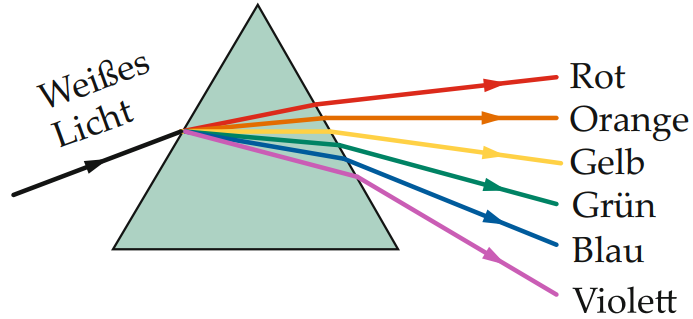
\includegraphics[width=0.50\linewidth]{Abbildungen Physik ZF/Dispersion.png}
\end{center}


\subsection{Polarisation}
EM-Wellen sind Transversalwellen \\[1ex]
- \textbf{lineare Polarisation:} Felder schwingen jeweils entlang einer Achse senkrecht \\ \hspace{5mm} zur Ausbreitungsrichtung \\[1ex]

- \textbf{zirkuläre Polarisation:} Die Spitzen der Feldvektoren beschreiben eine \\ \hspace{5mm} Spirale im Raum \\[2ex]

Mit \textbf{Polaristoren}, die nur eine bestimmte Schwingungsrichtung des $\Vec{E}-$Vektors durchlassen, lassen sich unpolarisierte Wellen linear polarisieren. \\[1ex]

\subsection{Polarisationsmechanismen}
\textbf{1. Absorption:} Richtungsabhängige Absorption in ausgerichteten linearen Molekülen oder Metallfäden, die nicht durchgelassene Polarisationsrichtung wird absorbiert \\ $\rightarrow$ Umwandlung in Wärme \\[1ex]
\textbf{Malusches Gesetz:}
\begin{formulabox}
    \[
        I_2 = I_1 \cos^2{\Theta}
    \]
\end{formulabox}

\textbf{2. Reflexion:} Wenn unpolarisiertes Licht bei einem bestimmten Winkel auf eine ebene Grenzfläche zwischen zwei durchsichtigen Medien triff, stehen der reflektierte und transmittierte Strahl senkrecht aufeinander. $\rightarrow$ reflektierte Welle wird vollständig linear polarisiert
\[
    n_1 \sin{\Theta_p} = n_2 \sin{\Theta_2} = n_2 \sin{(90^{\circ} - \Theta_p)} = n_2 \cos{\Theta_p}
\]
\textbf{Brewster Winkel}
\begin{formulabox}
    \[
        \tan{\Theta_p} = \frac{n_2}{n_1}
    \]
\end{formulabox}

\textbf{3. Streuung:} Reflexion und Absorption von EM-Wellen an Teilchen. Reemittiertes Licht, das in der Ebene senkrecht zur Einfallsrichtung gestreut wird, ist linear polarisiert.

\subsection{Lichtspektrum}
\textbf{Linienspektren:} Valenzelektronen sind für die Energieänderung im Atom zuständig, was zur Absorption führt. Die Energien des aus Atomen emittierten Lichts sind auf bestimmte Wellen beschränkt, was zu den diskreten Spektrallinien führt. \\[1ex]

\textbf{Kontinuierliche Spektren:} Wenn Atome stark miteinander wechselwirken, dann sind viele Energieniveaus der Atome zu ununterbrochenen Bereichen von Energieniveaus verbreitert. Daraus entsteht ein zusammenhängender Bereich \\
$\rightarrow$ kontinuierliches Emissionsspektrum \\[1ex]

\textbf{Sichtbares Licht:} Das menschliche Auge nimmt EM-Strahlung mit Wellenlängen zwischen $\approx 400nm \ - \ 700nm$ wahr. Die entsprechenden Photonenenergien liegen $\approx 1.8 eV \ - \ 3.1eV.$ Sonnenlicht, erscheint als weiss, da es Licht mit allen Wellenlängen in diesem Bereich ist.

			\section{Geometrische Optik}

\textbf{Grundlagen:}\\
\hspace{5mm} - geradlinige Ausbreitung von Licht (Lichtstrahlen) \\
\hspace{5mm} - Vernachlässigung von Wellenphänomenen (Beugung und Interferenz)

\subsection{Spiegel}

\textbf{Grundbegriffe:}
\begin{itemize}
	\item \textbf{virtuelles Bild:} Im Bildpunkt treffen sich nur die Verlängerungen der Strahlen
	\item \textbf{reelles Bild:} Im Bildpunkt treffen sich tatsächlich Lichtstrahlen
\end{itemize}

\textbf{Variablen:}
\begin{itemize}
	\item $G$: Gegenstandshöhe
	\item $g$: Gegenstandsweite
	\item $B$: Bildhöhe
	\item $b$: Bildweite
\end{itemize}

\textbf{Ebener Spiegel:} $G = B$, $g = b$ \\

\textbf{Sphärischer Spiegel:}
\begin{formulabox}
    \[
        \frac{1}{g} + \frac{1}{b} = \frac{2}{r}
    \]
\end{formulabox}
für $g \rightarrow \infty$ folgt: $b = \frac{r}{2} = f$: Brennweite des Spiegels \\
Parallel einfallende Strahlen fokussieren in der Brennebene \\
Achsenparallele Strahlen fokussieren im Brennpunkt \\[1ex]

\textbf{Bildkonstruktion bei sphärischen Spiegeln} \\
1. Der achsenparallele Strahl wird in den Brennpunkt reflektiert \\
2. Der Brennpunktstrahl verläuft durch den Brennpunkt und wird achsenparallel \\ \hspace{2.3mm} reflektiert \\
3. Der Mittelpunktstrahl verläuft durch den Krümmungsmittelpunkt, trifft den Spiegel und \\ \hspace{2.3mm} wird in sich selbst zurück reflektiert \\[1ex]

\textbf{Abbildungsmassstab:}
\begin{formulabox}
    \[
        V = \frac{B}{G} = -\frac{b}{g}
    \]
\end{formulabox}
$V > 0$ das Bild steht aufrecht\\
$V < 0$ das Bild ist invertiert \\[1ex]

\textbf{Vorzeichenregeln:} \\
1. $g$ ist positiv, wenn der Gegenstand auf der Seite des Spiegels ist, von der aus Licht \\ \hspace{2.3mm} auf den Spiegel trifft \\
2. $b$ ist positiv, wenn sich das Bild auf der Seite des Spiegels befindet, in die das Licht \\ \hspace{2.3mm} vom Spiegel reflektiert wird \\
3. $r$ (und daher auch $f$) ist positiv, wenn der Spiegel konkav ist. Dann liegt der \\ \hspace{2.3mm} Brennpunkt auf der Seite des Spiegels von der Licht einfällt 

\subsection{Linsen}
Ann.: Sphärische Grenzflächen zwischen zwei Medien mit Brechzahlen $n_1$ und $n_2$ \\[1ex]
\textbf{Brechung an einer Grenzfläche}
\begin{formulabox}
    \[
        \frac{n_1}{g} + \frac{n_2}{b} = \frac{n_2 - n_1}{r}
    \]
\end{formulabox}

\textbf{Vorzeichenkonvention für die Brechung:} \\
1. $g$ ist positiv, für Gegenstände auf der Einfallsseite der brechenden Fläche \\
2. $b$ ist positiv, für Bilder auf der Transmissionsseite der brechenden Fläche \\
3. $r$ ist positiv, wenn der Krümmungsmittelpunkt auf der Transmissionsseite der brechenden Fläche liegt

\subsection{Dünne Linsen}
\textbf{Für die Brechung an der ersten Grenzfläche gilt:}
\[
    \frac{n_{Luft}}{g} + \frac{n_{Linse}}{b_1} = \frac{n_{Linse} - n_{Luft}}{r_1}
\]
mit $\Rightarrow g_2 = -b_1$ folgt für die \textbf{Brechung an der zweiten Grenzfläche:}
\[
    \frac{n_{Linse}}{-b_1} + \frac{n_{Luft}}{b} = \frac{n_{Luft} - n_{Linse}}{r_2}
\]
\begin{formulabox}
    \[
        \frac{1}{g} + \frac{1}{b} = \left( \frac{n_{Linse}}{n_{Luft}} -1 \right) \left( \frac{1}{r_1} - \frac{1}{r_2} \right)
    \]
\end{formulabox}

\textbf{Reziproke Brennweite einer dünnen Linse:}
\begin{formulabox}
    \[
        \frac{1}{f} = \left( \frac{n_{Linse}}{n_{Luft}} -1 \right) \left( \frac{1}{r_1} - \frac{1}{r_2} \right)
    \]
\end{formulabox}

\textbf{Allgemeine Abbildungsgleichung:}
\begin{formulabox}
    \[
        \frac{1}{g} + \frac{1}{b} = \frac{1}{f}
    \]
\end{formulabox}

\textbf{Bildkonstruktion mit Linsen} \\
1. Der achsenparallele Strahl wird so gebrochen, dass er durch den zweiten \\ \hspace{2.3mm} Brennpunkt der Linse verläuft \\
2. Der Mittelpunktstrahl verläuft durch den Linsenmittelpunkt und wird nicht \\ \hspace{2.3mm} gebrochen (nur bei dünner Linse) \\
3. Der Brennpunktstrahl verläuft durch den ersten Brennpunkt und verlässt die \\ \hspace{2.3mm} Linse achsenparallel \\[1ex]

\textbf{Abbildungen mit mehreren Linsen} \\
Für zwei dünne Linsen auf derselben optischen Achse gilt:
\begin{formulabox}
    \[
        \frac{1}{f} = \frac{1}{f_1} + \frac{1}{f_2}
    \]
\end{formulabox}
Sie wirken wie eine dünne Linse mit der effektiven Brennweite $f$

			\section{Interferenz und Beugung}
\textbf{Interferenz:} Überlegung von Wellen, die statische Intensitätsmuster erzeugt. \\
\textbf{Beugung:} Abweichung der Wellenausbreitung von geometrischer Strahlrichtung an Öffnung oder Hindernis

\subsection{Phasendifferenz und Kohärenz}
Überlagerung zweier em-Wellen \\[1ex]
\hspace{5mm} $E_1 = E_0 \sin{(kx_1 - \omega t + \delta_1)}$ \\
\hspace{5mm} $E_2 = E_0 \sin{(kx_2 - \omega t + \delta_2)}$ \\[1ex]
\textbf{Differenz der Phasen beider Wellen} (zum Zeitpunkt $t$):

\begin{formulabox}
    \[
        (kx_1 - \omega t + \delta_1) - (kx_2 - \omega t + \delta_2) = k(x_1 - x_2) - \delta = k \cdot \Delta r - \delta
    \]
\end{formulabox}
    $\Delta r$: Wegunterschied / Gangunterschied \\[1ex]

\textbf{Konstruktive Interferenz:}
\[
    k \cdot \Delta r - \delta \hspace{3mm} \text{ganzzahliges Vielfaches von $2\pi$}
\]
\begin{center}
    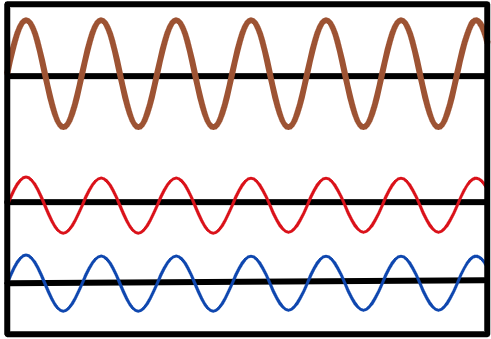
\includegraphics[width=0.18\linewidth]{Abbildungen Physik ZF/Konstruktive Interferenz.png}
\end{center}

\textbf{Destruktive Interferenz:}
\[
    k \cdot \Delta r - \delta \hspace{3mm} \text{unganzzahliges Vielfaches von $\pi$}
\]
\begin{center}
    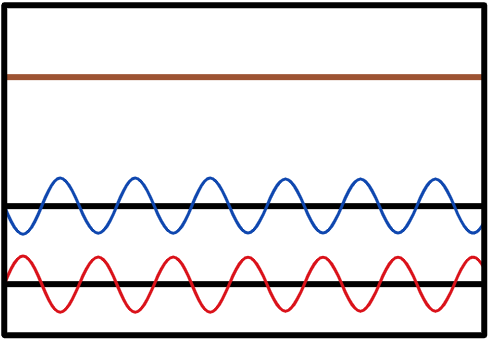
\includegraphics[width=0.18\linewidth]{Abbildungen Physik ZF/Destruktive Interferenz.png}
\end{center}

\textbf{Kohärenz:}
feste Phasenbezeichung \\
Allgemeiner: \textbf{"Interferenzfähigkeit"} \\
\hspace{5mm} Vorraussetzung: gleiche Polarisation \& Wellenlänge \\[1ex]

\subsection{Interferenz an dünnen Schichten}
\textbf{Phasenunterschied:}
\[
    \Delta = \frac{2 \pi}{\lambda'} \cdot 2s - \pi = \frac{2\pi}{\lambda} \cdot 2sn - \pi
\]

\textbf{Konstruktive Interferenz,} wenn:

\begin{formulabox}
    \[
        \Delta = m \cdot 2\pi \hspace{7mm} m = 0,  \pm 1, \pm 2, \dots
    \]
\end{formulabox}
    \hspace{5mm} $\rightarrow \lambda(m+\frac{1}{2}) = 2sn$ \\[1ex]
\textbf{Destruktive Interferenz,} falls:

\begin{formulabox}
    \[
        \Delta = (2m + 1)\pi \hspace{5mm} m = 0,  \pm 1, \pm 2, \dots
    \]
\end{formulabox}
    \hspace{5mm} $\rightarrow m\lambda = 2sn$ \\[1ex]

$\Rightarrow$ Streifenmuster durch Variation der Dicke $s$, \\ 
\hspace{3mm} bunte Streifen wegen Abhängigkeit von $\lambda$

\subsection{Interferenzmuster beim Doppelspalt}
Ann.: Die Wege des Lichts von den beiden Spalten zum Punkt $P$ auf dem Schirm können als parallel betrachtet werden. \\[1ex]
Für die Interferenz ist nur der Gangunterschied $d \cdot \sin{\Theta}$ entscheidend. \\[1ex]

\textbf{Intensitätsminima} (destruktiv):

\begin{formulabox}
    \[
        d \cdot \sin{\Theta} \Rightarrow \left(m + \frac{1}{2}\right) \lambda \hspace{5mm} m = 0,  \pm 1, \pm 2, \dots
    \]
\end{formulabox}

\textbf{Intensitätsmaxima} (kontruktiv):

\begin{formulabox}
    \[
        d \cdot \sin{\Theta} \Rightarrow  m\lambda \hspace{7mm} m = 0,  \pm 1, \pm 2, \dots
    \]
\end{formulabox}

\textbf{Für kleine Winkel $\Theta$ gilt:} $\sin{\Theta} = \tan{\Theta} = \frac{y}{l}$

\begin{formulabox}
    \[
        \Rightarrow y_m \approx m \cdot \frac{yl}{d} \hspace{5mm} \text{Position des m-ten Maximums}
    \]
\end{formulabox}

\textbf{Berechnung der Intensität auf dem Schirm:} \\[1ex]

\hspace{3mm} Welle von Spalt 1 zu Punkt $P$:
\[
    E_1 = A_0 \sin{\alpha} \hspace{10mm} \text{mit } \alpha = kx - \omega t
\]
\hspace{3mm} Welle von Spalt 2 zu Punkt $P$:
\[
    E_2 = A_0 \sin{(\alpha + \delta)} \hspace{7mm} \text{mit } \delta = k \cdot \Delta r = \frac{2\pi}{\lambda} \cdot d \sin{\Theta}
\]

\hspace{3mm} Aus \textbf{Überlagerung} resultierende Welle:

\begin{formulabox}
    \[
        E = E_1 + E_2  = \underbrace{2 A_0 \cos{ \left(\frac{1}{2}\delta \right)}}_{\text{Amplitude $E_0$ der Gesamtwelle}} \cdot \sin{\left( \alpha + \frac{1}{2}\delta \right)}
    \]
\end{formulabox}

\hspace{3mm} Intensität:

\begin{formulabox}
    \[
        I = |E_0|^2 = 4 A_0^2 \cos^2{\left(\frac{1}{2}\delta \right)}
    \]
\end{formulabox}

\subsection{Beugung am Gitter}
\textbf{Interferenzmaxima} zweier benachbarten Spalten liegen bei:

\[
    g \cdot \sin{(\Theta_m)} = m\lambda \hspace{7mm} m = 0,  \pm 1, \pm 2, \dots
\]

Das Gitter besitzt eine grosse Anzahl beleuchteter Spalten $N$. Das nächste Minium befindet sich dort, wo der Gangunterschied zwischen dem \textbf{mittleren Spalt $\frac{N}{2}$ und dem ersten Spalt $\frac{\lambda}{2}$} beträgt. (analog: 2. Spalt $\frac{N}{2} + 1$, usw.) \\[1ex]

\textbf{Der Abstand zwischen den beiden Spalten beträgt:}
\[
    \left( \frac{N}{2} - 1 \right) g \approx \frac{N}{2}g \hspace{10mm} \text{Ann.: $N$ ist gross} 
\]
\[
    \Rightarrow \frac{N}{2}\sin{(\Theta_{min})} = \frac{\lambda}{2} \hspace{10mm} \sin{(\Theta_{min}) \approx \Theta_{min} = \frac{\lambda}{N \cdot g}}
\]
\textbf{Breite der Maxima beim Gitter mit $N$ Spalten:}

\begin{formulabox}
    \[
        \Delta \Theta = 2 \Theta_{min} = \frac{2 \lambda}{N \cdot g}
    \]
\end{formulabox}
 
\hspace{5mm} $\rightarrow$ viele beleuchtete Spalten $\Rightarrow$ schmale Maxima \\
\hspace{5mm} $\Rightarrow$ gute Trennung unterschiedlicher Wellenlängen \hspace{1mm} (Anwendung: Spektrometer)

\subsection{Beugung beim Einzelspalt}
Im Intensitätsminimum löschen sich der Mittelstrahl und ein Strahl vom Rand des Spalts gegenseitig aus. Daraus folgt: 

\[
    \underbrace{\frac{1}{2}a  \cdot \sin{(\Theta_1)}}_{\text{Gangunterschied}} = \underbrace{\frac{1}{2}\lambda}_{\text{Bedingung für destruktive Interferenz}}
\]

\begin{formulabox}
    \[
        \sin{(\Theta_1)} = \frac{\lambda}{a}
    \]
\end{formulabox}

\textbf{Analog findet man für die weiteren Minima:}

\begin{formulabox}
    \[
        \sin{(\Theta_m)} = m \frac{\lambda}{a} \hspace{7mm} m = 0,  \pm 1, \pm 2, \dots
    \]
\end{formulabox}

\subsection{Beugung und Auflösung}
\textbf{Betrachtung:} Beugung an einem kreisrunden Öffnung mit Durchmesser $D$ \\[1ex]

Winkel unter dem das \textbf{erste Intensitätsminimum auftritt:}

\begin{formulabox}
    \[
        \sin{(\Theta)} = 1.22 \frac{\lambda}{D}
    \]
\end{formulabox}

\textbf{Für kleine Winkel:}

\begin{formulabox}
    \[
        \Theta = 1.22 \frac{\lambda}{D} \hspace{5mm} \text{oder. } \frac{x}{h}
    \]
\end{formulabox}

Dient als Kirterium für das Auflösungsvermögen eines Instruments \textbf{(Rayleigh Kriterium)}

			\newpage
			
			\section{Anmerkung vom Verfasser}
\begin{flushleft}

Diese Zusammenfassung wurde von \textbf{Stephan Wyss} für die Vorlesung \textit{Physik} von Dr. Prof. Lukas Gallmann (Frühjahrssemester 2026) erstellt. \\[3ex]

\textbf{\textcolor{red}{Hinweis:}} Richtigkeit und Vollständigkeit kann \textbf{nicht garantiert} werden. \\[5ex]

\textbf{Viel Erfolg, ihr packt das!}

\columnbreak

\end{flushleft}
			\begin{minipage}{\columnwidth}
	\section{Änderungsprotokoll}
\begin{tabular}{p{0.2\linewidth} | p{0.7\linewidth}}
	01.06.2026 & \textbullet~ Veröffentlichung der originalen Version (DE) \\[1.5ex]
	05.06.2026 & \textbullet~ Anpassung Ladung Protonen zu positiv e \newline 
	\textbullet~ Korrektur bei Zyklonperiode von $|1 \cdot B|$ zu $|q \cdot B|$ \newline
	\textbullet~ $U = \frac{g \cdot d}{\epsilon_0 \cdot A}$ zu $U = \frac{q \cdot d}{\epsilon_0 \cdot A}$ korrigiert \newline
	\textbullet~ E-Feld ausserhalb der Oberfläche zu E-Feld zwischen den Oberflächen geändert \newline
	\textbullet~ $\sin{\Theta_k} = \frac{n_1}{n_2}\sin{90^{\circ}} = \frac{n_2}{n_1}$ zu $\frac{n_2}{n_1}\sin{90^{\circ}}$ korrigiert \newline
	\textbullet~ Auftreffen auf ein Medium bei Totalreflexion und nicht Eintreten \newline
	\textbullet~ Kapitel zu Konstanten und Einheiten hinzugefügt
\end{tabular}
\end{minipage}

			
			% End the layout structure before closing the document
		\end{adjustwidth}
	\end{multicols*}
	
\end{document}